\section{Task Planning and Execution}
\label{sec:decision_making}

Once the customer submits an order, the Task Planner creates
a plan to collect the items in the order throughout the store and bring the shopping basket to the delivery location.

Our decision-making approach to creating these plans and executing them is designed explicitly with failure recovery in mind. It consists of i) offline plans that leverage the known structure of the task, and ii) online planning to adapt the sequence of actions to unforeseen disturbances, following the approach in \cite{pezzato2023active}. Offline planning involves planning a sequence of desired states as leaf nodes in a behavior tree --- instead of the standard action nodes--- to send task sub-goals to the online active inference planner. The latter is an online planner that computes an action sequence to transition from the current state to the next desired one.

\subsubsection{Offline planning}

The structure of the task is modelled offline as a plan to be executed using the template behavior tree shown in Fig.~\ref{fig:bt_full} and expanded by Fig.~\ref{fig:subtree}, making the robot try to pick every product up to $N$ times, and then deliver the groceries to the delivery location.
It specifies an initial welcome to the customer, a ``Product Subtree'' slot, an active inference node that sets the final task sub-goal of being at the delivery location for the online active inference planner, and a closing message to the customer.  For each product, a sub-tree as in Fig.~\ref{fig:subtree} is created automatically. Following the ordered list, every sub-tree for each product is inserted in the overall BT structure from Fig.~\ref{fig:bt_full}, as part of the sequence.
%The overall BT will  


\begin{figure}[b!]
    \centering
    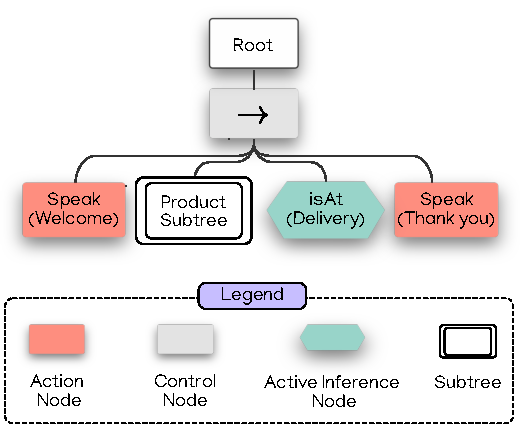
\includegraphics[width=0.8\linewidth]{bt_full.pdf}
    \caption{Overall Behavior Tree structure. The action \texttt{Speak{}} interfaces with the voice module to produce a suitable message for the customers (see Sec.~\ref{sec:teaching}).}
    \label{fig:bt_full}
\end{figure}



\begin{figure}[b!]
    \centering
    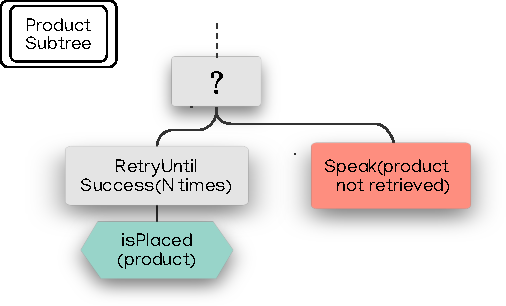
\includegraphics[width=0.8\linewidth]{bt_subtree.pdf}
    \caption{Sub-tree structure for placing an item in the basket. The active inference node sets a prior over the state \texttt{isPlaced{}} for a product, triggering the online decision-making. The action \texttt{Speak{}} produces a voice message to explain the failure in case one happens (see Sec.~\ref{sec:teaching}).}
    \label{fig:subtree}
\end{figure}




\subsubsection{Online planning with Active Inference} 

The active inference planner (AIP) takes the task sub-goals \texttt{isPlaced} and \texttt{isAt} as desired states of items being placed in the robot's basket and the robot being at the delivery location respectively, and computes a plan of symbolic actions based on the robot's skills that achieves those states.
Our planner is based on discrete active inference, which relies on a generative model that contains beliefs about future states and action plans, where plans that lead to preferred states are more likely. The preferred action sequence is the one with the highest probability of achieving desired states. 

Our active inference planner rests on the tuple $(\mathcal{O},\mathcal{S},\mathcal{A})$. This is composed of a finite set of observations $\mathcal{O}$, a finite set of symbolic states $\mathcal{S}$, and a finite set of symbolic actions $\mathcal{A}$ that correspond to the robot's skills.


The continuous state of the world $x\in\mathcal{X}$ is discretized through a symbolic observer into boolean variables about the relevant states of the world, e.g., item held by the gripper. These discrete observations $o$ are used to build a probabilistic belief about the symbolic current state, described in Table~\ref{tab:States}.



The AIP computes the posterior distribution over $p$ plans $\bm \pi$ through free-energy minimization \cite{pezzato2023active}. The symbolic action to be executed by a robot in the next time step is the first action of the most likely plan, denoted with $\pi_{\zeta, 0}$:
\begin{eqnarray}
\label{eq:a_t}
    \zeta = \max(\underbrace{[\bm\pi_{1}, \bm\pi_{2},...,\bm\pi_{p}]}_{\bm \pi^\top}),\ 
    a_{\tau=0} = \pi_{\zeta, 0}.
\end{eqnarray}




\begin{table}[ht!]
\caption{Notation for states}% title of Table
\centering % used for centering table
%\begin{tabular}{C{2.8cm} C{4.7cm}} % 
\begin{tabular}{c c} % 
\toprule %inserts double horizontal lines
\textbf{State, Boolean State} & \textbf{Description}\\ [0.5ex] % 
\midrule % inserts single horizontal line
${s^{(at)}},\ {l^{(at)}}$ & Belief about being at the goal location \\
${s^{(loc)}},\ {l^{(loc)}}$ & Belief about being self-localized \\
${s^{(reach)}},\ {l^{(reach)}}$ & Belief about reachability of an object\\
${s^{(hold)}},\ {l^{(hold)}}$ & Belief about holding an object\\
${s^{(vis)}},\ {l^{(vis)}}$ & Belief about an object being in sight\\
${s^{(place)}},\ {l^{(place)}}$ & Belief about an object being placed at a location\\
\midrule
\textbf{Boolean State} & \textbf{Common Name}\\ [0.5ex] % 
\midrule % inserts single horizontal line
${l^{(at)}= [1\ 0]^\top}$ & \texttt{isAt(goal\slash obj)} \\
${l^{(loc)}= [1\ 0]^\top}$ & \texttt{isLocalized} \\
${l^{(reach)}= [1\ 0]^\top}$ & \texttt{isReachable(obj)}\\
${l^{(hold)}= [1\ 0]^\top}$ & \texttt{isHolding(obj)}\\
${l^{(vis)}= [1\ 0]^\top}$ & \texttt{isVisible(obj)}\\
${l^{(place)}= [1\ 0]^\top}$ & \texttt{isPlaced(obj)}\\
\bottomrule %inserts single line
\end{tabular}
\label{tab:States}
\end{table}

% \begin{table}[ht!]
% \caption{Common name for states}% title of Table
% \centering % used for centering table
% \begin{tabular}{C{3cm} C{3cm}} % 
% \toprule %inserts double horizontal lines
% \textbf{Boolean State} & \textbf{Common Name}\\ [0.5ex] % 
% \midrule % inserts single horizontal line
% ${l^{(at)}= [1\ 0]^\top}$ & \texttt{isAt(goal\slash obj)} \\
% ${l^{(loc)}= [1\ 0]^\top}$ & \texttt{isLocalized} \\
% ${l^{(reach)}= [1\ 0]^\top}$ & \texttt{isReachable(obj)}\\
% ${l^{(hold)}= [1\ 0]^\top}$ & \texttt{isHolding(obj)}\\
% ${l^{(vis)}= [1\ 0]^\top}$ & \texttt{isVisible(obj)}\\
% ${l^{(place)}= [1\ 0]^\top}$ & \texttt{isPlaced(obj)}\\
% \bottomrule %inserts single line
% \end{tabular}
% \label{tab:common_names}
% \end{table}

\begin{table}[h]
\caption{Notation for actions}% title of Table
\centering % used for centering table
\begin{tabular}{p{2.5cm}p{2.5cm}p{2.5cm}} % centered columns (4 columns)
\toprule
    \textbf{Actions}& \textbf{Preconditions}& \textbf{Postconditions}\\ 
    \midrule
    \texttt{selfLoc()} & \texttt{-} & \texttt{isLocalized} \\
    \texttt{moveTo(goal\slash obj)} & \texttt{isLocalized} & \texttt{isAt(goal)}\slash \\
    & & \texttt{isReachable(obj)} \\  
    \texttt{pick(obj)} & \texttt{isReachable(obj)}& \texttt{isHolding(obj)}\\ 
     & \texttt{!isHolding} & \\
     & \texttt{isVisible(obj)} & \\
    \texttt{place(obj)} & \texttt{isHolding}& \texttt{isPlaced(obj)}\\
    &  & \texttt{!isHolding(obj)}\\
    \texttt{look(obj)} & \texttt{-} & \texttt{isVisible(obj)}\\
    \bottomrule
\end{tabular}
\end{table}
%
%\CP{postconditions naming and isAt etc should match}
%

The combination of offline plans modelled as behaviour trees and online planning using active inference facilitates responsive action selection for long-term tasks within partially observable and dynamic environments, which is particularly crucial in addressing disturbances in retail settings. 

 This approach offers the advantage of not having to account for every conceivable contingency and recovery behavior within a Behavior Tree, and at the same time allows for continuous online planning.
 This effectively minimizes computational complexity, enabling the development of a robot capable of adhering to predefined routines while also adapting locally to unforeseen events through real-time online planning with active inference.
